\documentclass{standalone}
\usepackage{currfile}
\usepackage[mode=buildnew]{standalone}
\usepackage{tikz}
\usetikzlibrary{trees}

\begin{document}
	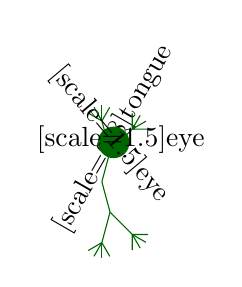
\begin{tikzpicture}
		\node[draw=none,fill=none,rotate=60] at (0.15,0.55) {\includestandalone[scale=0.8]{\currfiledir tongue}};
		\begin{scope}
			[draw=green!40!black, grow cyclic, 
			level 1/.style={level distance=4mm,sibling angle=150},
			level 2/.style={level distance=4mm,sibling angle=60},
			level 3/.style={level distance=2mm,sibling angle=30}]
			\coordinate [rotate=-90] % going down
			child foreach \x in {1,2}
			{child foreach \x in {1,2}
				{child foreach \x in {1,2,3,4}}};
		\end{scope}
		\fill[green!40!black] (0.15,0.5) circle (0.2cm);
		\node[draw=none,fill=none,rotate=-50] at (0.1,0.6) {\includestandalone[scale=1.5]{\currfiledir eye}};
		\node[draw=none,fill=none] at (0.24,0.53) {\includestandalone[scale=1.5]{\currfiledir eye}};
	\end{tikzpicture}
\end{document}
